\documentclass[SensorSystemsProject.tex]{subfiles}

%Implementation issues (document only what is not documented in the selected literature, but necessary for implementation, e.g. software structure…)

\begin{document}
\chapter{Implementation issue}
\section{Color based face detection on a picture}
To load an image into the workspace and find suitable thresholds in the YCbCr space the informations from the lecture \textit{Color} in the course \textit{Image and Signal Processing} (\cite{RobAmaColor}). A detailed description to this procedure can be found in the attachment \ref{sec:ColorThre}

\medskip
The thresholding itself can be done by logical operations like in the listening \ref{matlabColorTresholdingDetail}.

\begin{lstlisting}[caption=Color thresholding, label= matlabColorTresholdingDetail]
% Thresholding -> binary
thresh_cb = cb > 105 & cb < 120;    % thresholding for cb values
thresh_cr = cr > 140 & cr < 165;    % thresholding for cr values
binary_pic = thresh_cb&thresh_cr;   % create binary picture
\end{lstlisting}

\medskip
To detect faces out of the binary image (to reject areas/blobs which are no faces) a few process steps are necessary. The process is described in the article \cite{RTFaceDetection}.
To verify that the found skin region represents a face, it must satisfy every of the following conditions:

\paragraph{Small Area} Skin regions which have less than a specified number of pixels are rejected. This number highly depends on the resolution of the image and has to be defined individually for each resolution.
\paragraph{Euler Number} Human faces contain some holes like eyes, eyebrows, a mouth etc. If a skin region does not contain any holes, this region is discarded. This is done using the Euler Number:	$E = C – H$. Where C is the number of connected components and H is the number of holes in a region. If the Euler Number is greater than zero, the region is discarded.
\paragraph{Eccentricity} The oval shape of a face can be approximated by an ellipse. If a skin region has an eccentricity greater than 0.91, it gets discarded. An ellipse whose eccentricity is 0 is a circle, while an ellipse whose eccentricity is 1 represents a line segment.

\paragraph{Bounding Box Properties} If height to width ratio of a skin region is greater than $\frac{1}{2}$, the skin region is discarded. 

\medskip
The used values for the eccentricity and the bounding box condition are obtained by trial and error. For the implementation of these conditions ready-made MATLAB-Functions are available. The code can be seen in listing  \ref{RejectionOfNonSkinRegion}.

\begin{lstlisting}[caption=Rejection of non Face Skin Region , label= RejectionOfNonSkinRegion]
%label all the connected components in the image
bw=bwlabel(close_binary_pic,8);

%image blob analysis - we get a set of properties for each labeled region
area=regionprops(bw,'Area')                    
eulernumber=regionprops(bw,'EulerNumber');      
eccentricity=regionprops(bw,'Eccentricity');    
centroid=regionprops(bw,'Centroid');            
boundingbox=regionprops(bw,'BoundingBox');
\end{lstlisting}

After applying the above mentioned conditions to the binary image, rectangles are drawn around the remaining skin regions. This can be seen in figure \ref{detectedFaces}.

\begin{figure}[!h]
\centering
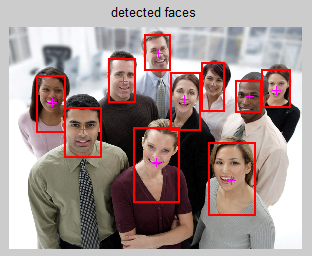
\includegraphics[width=10cm]{./img/faceDetectionPicture/detectedFaces.png} 
\caption{Detected faces}
\label{detectedFaces}
\end{figure}

\paragraph{Computation time} The computation time of the face detection algorithm highly depends on the size of the image and the detected skin area. The image shown in figure \ref{detectedFaces} for example has a size of 1548x2048 pixels and needs a computation time of 1.241 seconds using the MATLAB stopwatch timer. 
Considering the fact that the MATLAB plot functions need a lot of computation time, the measurement was repeated without plotting. The algorithm then needs 0.923 seconds computation time.

\medskip
The whole script can be found in the attachment \ref{DetectionOnAPicture}.


\section{Color based face detection on a video}
After implementing face detection on images, the algorithm is now enhanced to detect faces in a webcam video stream. 

The main idea is to take snapshots of the incoming video stream to let them run through the former explained algorithm for face detection in images. Every time the acquired image is fully processed, a new snapshot is taken. 

Knowing that the computation time of the algorithm highly depends on the size of the image, the resolution is set to 320x240 pixel. Thus it can be guaranteed that the algorithm is fast enough for real time applications.

\paragraph{Calculation time}
The calculation time for processing a snapshot and plotting the image with rectangles around faces lies in between 0.04 and 0.09 seconds. Taking the snapshot takes another 0.08 - 0.1 seconds. 
Corresponding to this values, the algorithm has a worst-case computation time of 0.19 seconds and a best-case computation time of 0.12 seconds for each snapshot. In other words the frames per second rate lies in between 5.26 and 8.33 (see table \ref{performanceComparison}).

\begin{table}[!h]
\centering
	\begin{tabular}{|l|c|c|}
	\hline 
	ID & Best case & Worst case \\ 
	\hline 
	Computation time for on snapshot & 0.12 s & 0.19 s \\ 
	\hline 
	Frames per second	&8.33	&5.26\\
	\hline
	\end{tabular} 
\caption{Performance comparison}
\label{performanceComparison}
\end{table}


The whole script for the face detection on a video using MATLAB can be found in appendix \ref{DetectionOnAVideo}.



\section{Color based face detection on a Raspberry Pi}

\subsection{Simulink Model - Face detection on an image}
The \textit{Image Processing Toolbox } from Simulink provides the function to load an image from a file, convert this image (from RGB) into the YCbCr space, make the blob analysis, draw the rectangular (which represents a detected face) on the image and display the image on a figure. 

To threshold the YCbCr image a MATLAB-function block (\textit{color thresholding} in figure \ref{SimulinkImage}) was inserted. The MATLAB-function block \textit{remove misshapen skin regions} is used to remove rectangles which are wider than height (with this functions skin regions from vertical hands can be rejected). This function block was necessary because the Blob Analysis block didn't support all necessary functions (for example the eulernumber is missing).

\begin{figure}[!h]
\centering
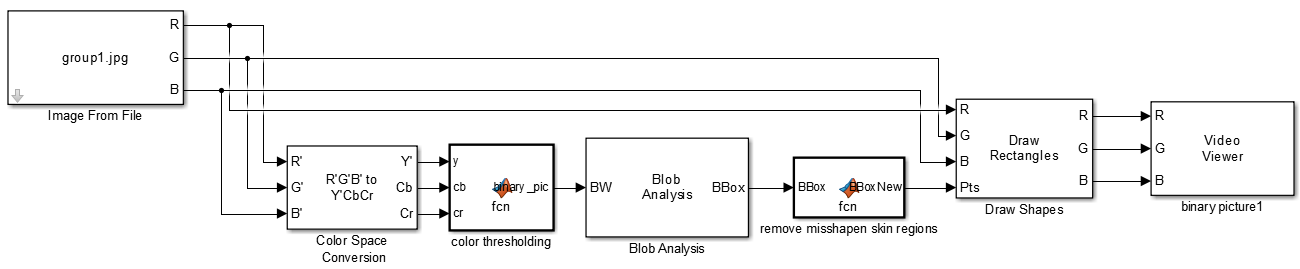
\includegraphics[width=14cm]{./img/simulink/Simulink_ImageProcessing.PNG} 
\caption{Simulink model - Face detection on an image}
\label{SimulinkImage}
\end{figure}

The code of the Matlab function blocks can be found in the attachment \ref{sec:SimulinkFaceImage}.


\subsection{Simulink Model deployed on Raspberry Pi with I/O connection to the host PC}

To run a Simulink model on a Raspberry Pi the hardware support package Run models on Raspberry Pi is necessary. The package installation hints and Examples can be found on \href{https://de.mathworks.com/hardware-support/raspberry-pi-simulink.html}{Raspberry Pi Support from Simulink}. 

\medskip
Hints to run a Simulink block on the Raspberry Pi:
\begin{itemize}
\item Use a standalone licence or a network licence without VPN. By using a licence over a VPN it is not possible to communicate with the Raspberry Pi.
\item Before using the Raspberry Pi camera module the steps from the instructions \href{https://de.mathworks.com/help/supportpkg/raspberrypi/ug/add-support-for-raspberry-pi-camera-board.html}{Use Camera Board with V4L2 Video Capture Block} must be done. Otherwise the Simulink block will not find the camera module.
\end{itemize}


\medskip
In a first step the setup looks like figure \ref{SetupWithIO}. The idea is to get familiar with the Raspberry Pi camera module (the resolution, brightness, ...) and use the data for adjustments (especially for find suitable thresholds). In this case the model should run in the external mode, the instructions \href{https://de.mathworks.com/help/supportpkg/rtlsdrradio/ug/run-model-in-external-mode.html}{Run Model in External Mode} provides all necessary informations.

\begin{figure}[!h]
\centering
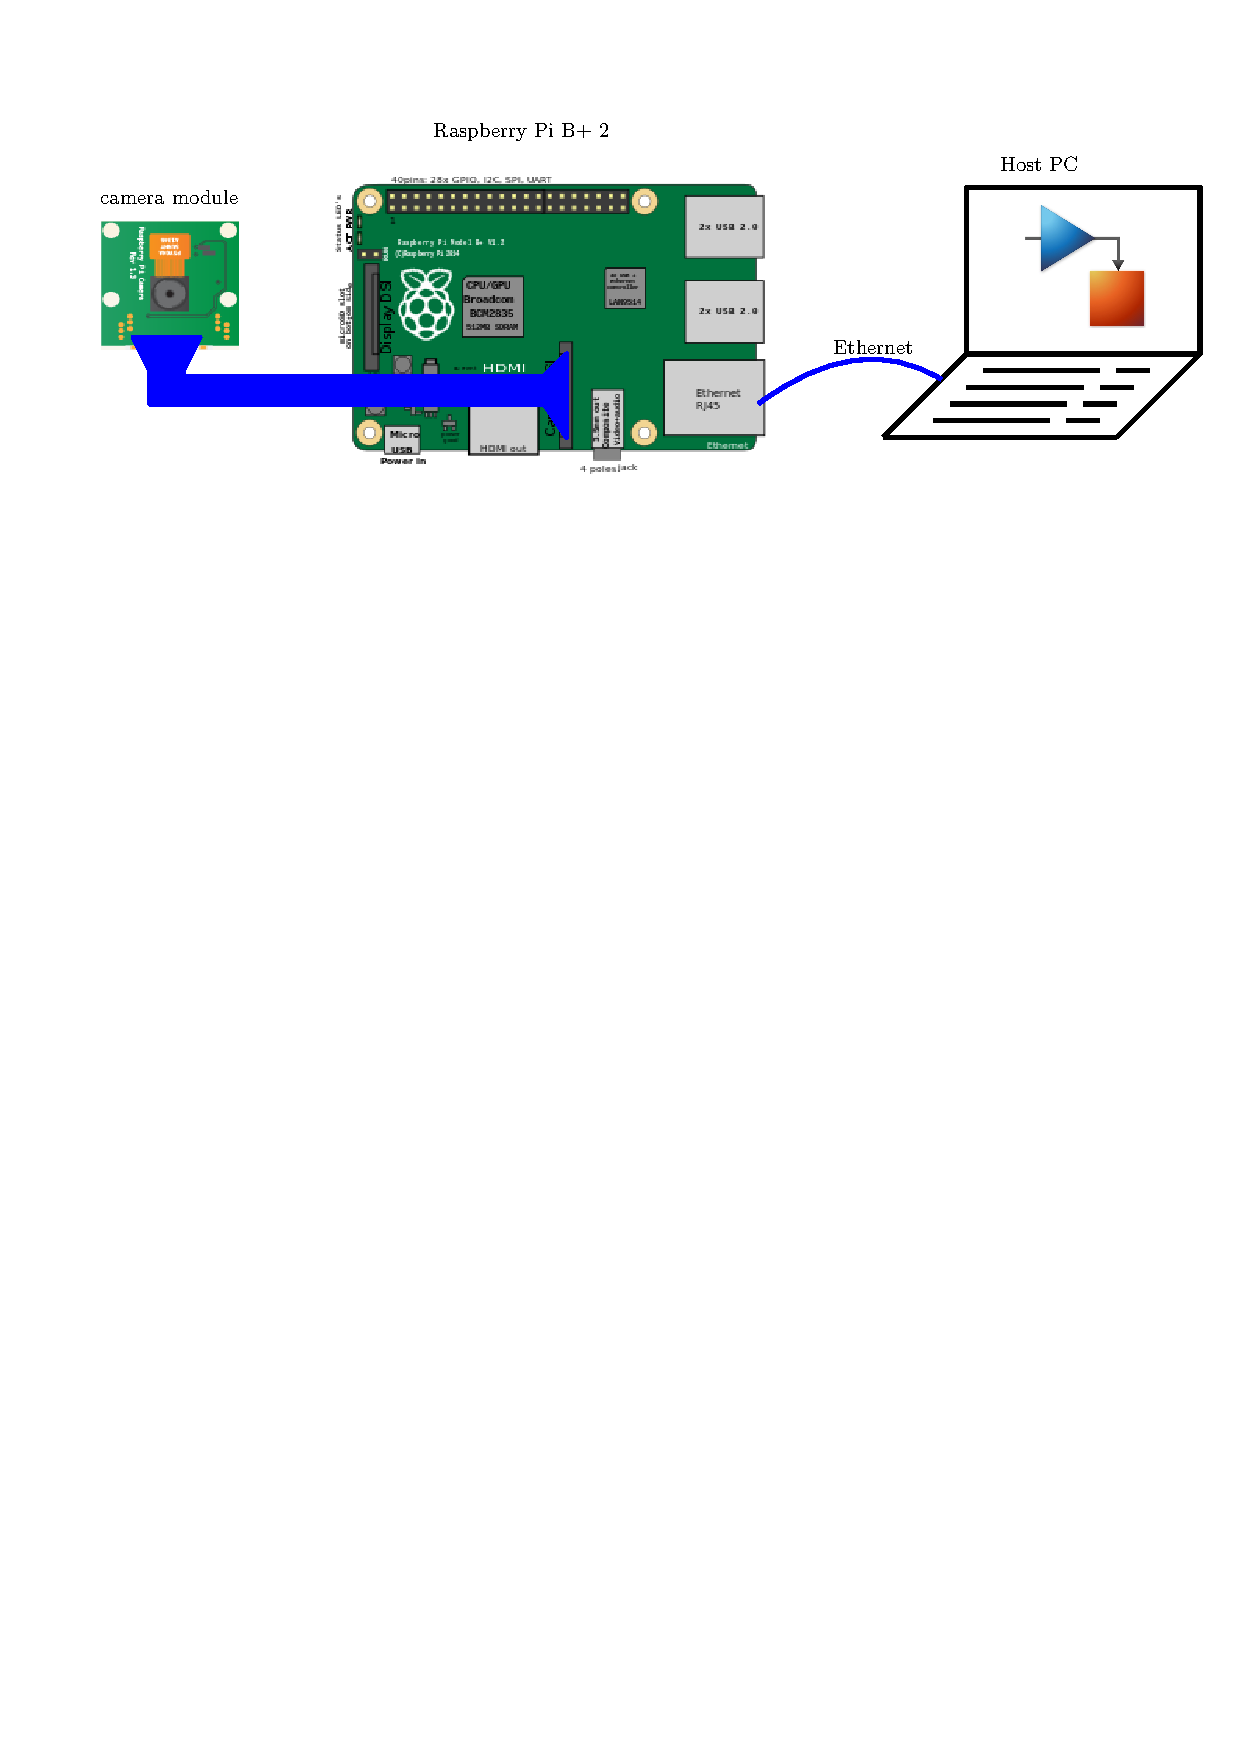
\includegraphics[page=1,width=14cm]{./img/raspberryPi/setups.pdf} 
\caption{Simulink model setup - With I/O connection to the host}
\label{SetupWithIO}
\end{figure}

The Simulink model itself was built up similar with the model in figure \ref{SimulinkImage}, see figure \ref{SimModelRaspIO_safsdf}.

\begin{figure}[!h]
\centering
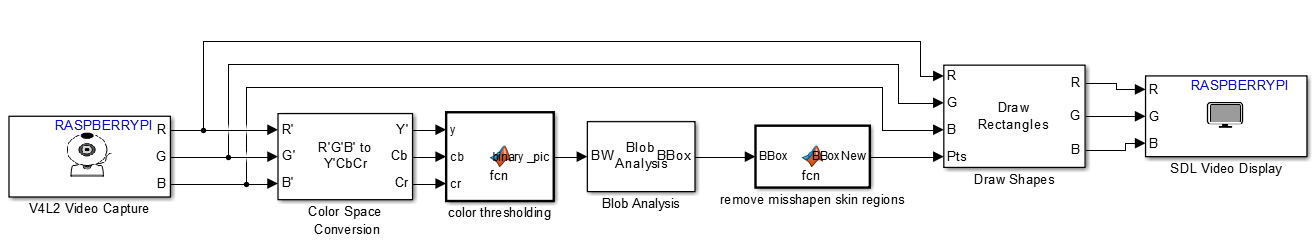
\includegraphics[width=14cm]{./img/simulink/Simulink_RaspberryPi.PNG} 
\caption{Simulink model - With I/O connection to the host}
\label{SimModelRaspIO_safsdf}
\end{figure}

\subsection{Simulink Model as Standalone Application}
The final step is to deploy the on the hardware like in figure \ref{SimModelStandalone}. As model the model of figure \ref{SimModelRaspIO_safsdf}. To deploy the model on the hardware the instruction \href{https://de.mathworks.com/help/supportpkg/rtlsdrradio/ug/run-model-as-standalone-application.html}{Run Model as Standalone Application} is useful.

\begin{figure}[!h]
\centering
\includegraphics[page=2,width=14cm]{./img/raspberryPi/setups.pdf} 
\caption{Simulink model setup - Standalone application}
\label{SimModelStandalone}
\end{figure}




\end{document}
